% % % % % % % % % % % % % % % % % % % % % % % % % % % % % % % % % % % % % % % %
% LaTeX4EI Template for Cheat Sheets                                Version 1.1
%
% Authors: Emanuel Regnath, Martin Zellner
% Contact: info@latex4ei.de
% Encode: UTF-8, tabwidth = 4, newline = LF
% % % % % % % % % % % % % % % % % % % % % % % % % % % % % % % % % % % % % % % %


% ======================================================================
% Document Settings
% ======================================================================

% possible options: color/nocolor, english/german, threecolumn
% defaults: color, english
\documentclass[english]{latex4ei/latex4ei_sheet}
\usepackage{empheq}
\usepackage{gensymb}
\usepackage{tikz}
\usetikzlibrary{arrows.meta,calc,angles,positioning}


% set document information
\title{LaTeX4EI \\ Cheat Sheet}
\author{LaTeX4EI}					% optional, delete if unchanged
\myemail{info@latex4ei.de}			% optional, delete if unchanged
\mywebsite{www.latex4ei.de}			% optional, delete if unchanged


% ======================================================================
% Begin
% ======================================================================
\begin{document}

% Title
% ----------------------------------------------------------------------
\maketitle   % requires ./img/Logo.pdf

% Section
% ----------------------------------------------------------------------



\section{Einheiten}

\begin{sectionbox}
	\subsection{SI-Präfixe}
	
	\begin{tablebox}{ccl|ccl}
		Symbol & Präfix & Faktor & Symbol & Präfix & Faktor \\
		\hline
		Q  & Quetta & $10^{30}$ & d & Dezi & $10^{-1}$\\
		R  & Ronna  & $10^{27}$ & c & Zenti & $10^{-2}$\\
		Y  & Yotta  & $10^{24}$ & m & Milli & $10^{-3}$\\
		Z  & Zetta  & $10^{21}$ & µ & Mikro & $10^{-6}$\\ 
		E  & Exa    & $10^{18}$ & n & Nano  & $10^{-9}$\\
		P  & Peta   & $10^{15}$ & p & Piko  & $10^{-12}$\\
		T  & Tera   & $10^{12}$ & f & Femto  & $10^{-15}$\\
	 	G  & Giga   & $10^9$    & a & Atto   & $10^{-18}$\\
		M  & Mega   & $10^6$    & z & Zepto  & $10^{-21}$\\
		k  & Kilo   & $10^3$    & y & Yokto  & $10^{-24}$\\
		h  & Hekto  & $10^2$    & r & Ronto  & $10^{-27}$\\
		da & Deka   & $10^1$    & q & Quekto & $10^{-30}$\\
	\end{tablebox}

	\subsection{Binäre Präfixe}
	
	\begin{tablebox}{ccll}
		Symbol & Präfix & Faktor & Dez. Äquiv. \\
		\hline			
		Ki & Kibi  & $2^{10}$  & $= 1.024e3$ \\
		Mi & Mebi  & $2^{20}$  & $≈ 1.049e6$ \\
		Gi & Gibi  & $2^{30}$  & $≈ 1.074e9$ \\
		Ti & Tebi  & $2^{40}$  & $≈ 1.100e12$ \\
		Pi & Pebi  & $2^{50}$  & $≈ 1.126e15$ \\
		Ei & Exbi  & $2^{60}$  & $≈ 1.152e18$ \\
		Zi & Zebi  & $2^{70}$  & $≈ 1.181e21$ \\
		Yi & Yobi  & $2^{80}$  & $≈ 1.209e24$ \\
		Ri & Robi  & $2^{90}$  & $≈ 1.238e27$ \\
		Qi & Quebi & $2^{100}$ & $≈ 1.268e30$ \\
	\end{tablebox}

	\subsection{SI-Einheiten}

	\begin{tablebox}{llc}
		Grösse & Einheit & \\
		\hline
		Länge & Meter & m \\
		Masse & Kilogramm & kg \\
		Zeit & Sekunde & s \\
		Stromstärke & Ampere & A \\
		Temperatur & Kelvin & K \\
		Stoffmenge & - & mol \\
		Lichtstärke & Candela & cd			
	\end{tablebox}	
	
	\subsection{Abgeleitete Einheiten}

	\begin{tablebox}{lcllc}
		Grösse & Sym. & Einheit &  & SI \\
		\hline
		Kraft & F & Newton & N & $kg\cdot m/s^2$ \\
		Energie/Arbeit & E/W & Joule & J & $Nm$ \\
		Leistung & P & Watt & W & $J/s$ \\
		El. Ladung & Q & Coulomb & C & $A \cdot s$ \\
		El. Potential & $\phi$ & Volt & V & $J/C$ \\
		Spannung & U & Volt & V & $J/C$ \\
		El. Widerstand & R & Ohm & $\ohm$ & $V/A$ \\
		El. Leitwert & G & Siemens & S & $A/V$ \\
		Spez. el. Widerstand & $\rho$ & - & - & $Ωm$ \\
		Spez. el. Leitwert & $\gamma$ & - & - & $S/m$ \\
		El. Feldstärke & E & - & - & $V/m$ \\
		El. Stromdichte & J & - & - & $A/m^2$ \\
	\end{tablebox}
		
\end{sectionbox}

\section{Elektrotechnik}
	
\begin{sectionbox}
	\subsection{Ohmsches Gesetz}

	\begin{emphbox}
	Ohmsches Gesestz: $ U = R \cdot I = \frac{I}{G} $
	\end{emphbox}

	\subsection{Leistung}

	\begin{emphbox}
	$ P = U \cdot I = \frac{U^2}{R} = I^2 \cdot R $
	\end{emphbox}
	

		
\end{sectionbox}

\begin{sectionbox}
	\subsection{Kirchoffsche Gesetze}

	Knotenregel:
	\begin{emphbox}
		In einem Knoten: Summe der zufliessenden Ströme = Summe der abfliessenden Ströme\\
		$\sum _{k=1}^{n}I_k = 0$
	\end{emphbox}
	
	Maschenregel:
	\begin{emphbox}
		In einer Masche: Summe der Teilspannungen addieren sich zu Null. Pfeilrichtungen beachten!\\
		$\sum _{k=1}^{n}U_k = 0$
	\end{emphbox}

\end{sectionbox}


\begin{sectionbox}
	\subsection{Widerstand}

	\begin{emphbox}
	Leitwert:	$ G = \frac{1}{R} $\\
	\end{emphbox}	
	
	Parallelschaltung:
	\begin{emphbox}
		\begin{align*}
			\frac{1}{R_{tot}} &= \sum _{k=1}^{n}\frac{1}{R_k} &= \frac{1}{R_{1}} + \frac{1}{R_{2}} + \ldots + \frac{1}{R_k}\\
			G_{tot} &= \sum _{k=1}^{n}G_k &= G_1 + G_2 + \ldots + G_k
		\end{align*}
	\end{emphbox}
	
	Serieschaltung:
	\begin{emphbox}
			\begin{align*}
			R_{tot} &= \sum _{k=1}^{n}R_k &= R_1 + R_2 + \ldots + R_k
		\end{align*}

	\end{emphbox}

	
\end{sectionbox}


\begin{sectionbox}
	\subsection{Kondensator}

	Lade-/Entladevorgang:
	\begin{emphbox}
		\begin{align*}
			u_C(t) &= U_0+ ΔU \cdot e^{-{\frac{t}{τ}}} = U_0+ (U_{C,t0}-U_0) \cdot e^{-{\frac{t}{τ}}} \\
			i_C(t) &= \frac{u_C(t)}{R_C} = \frac{U_0}{R_C}+\frac{ΔU}{R_C}\cdot e^{-{\frac{t}{τ}}}
		\end{align*}
	\end{emphbox}

	Ladevorgang:
	\begin{emphbox}
		\begin{align*}
			u_C(t) &= U_0 \cdot (1-e^{-{\frac{t}{τ}}}) \\
			i_C(t) &= I_0 \cdot e^{-{\frac{t}{τ}}}
		\end{align*}
	\end{emphbox}

	Entladevorgang:
	\begin{emphbox}
		\begin{align*}
			u_C(t) &= U_0 \cdot e^{-{\frac{t}{τ}}} \\
			i_C(t) &= -I_0 \cdot e^{-{\frac{t}{τ}}}
		\end{align*}
	\end{emphbox}

mit
\begin{emphbox}
	$I_0 = \frac{U_0}{R_C}$
	
	$τ = R_C \cdot C$
\end{emphbox}

	
\end{sectionbox}

\begin{sectionbox}
	\subsection{Spule}

Lade-/Entladevorgang:
\begin{emphbox}
	$u_C(t) = U_0+ ΔU \cdot e^{-{\frac{t}{τ}}} = U_0+ (U_{C,t0}-U_0) \cdot e^{-{\frac{t}{τ}}} ???$

	$i_C(t) = \frac{u_C(t)}{R_C} = \frac{U_0}{R_C}+\frac{ΔU}{R_C}\cdot e^{-{\frac{t}{τ}}} ???$
\end{emphbox}

Ladevorgang:
\begin{emphbox}

	$i_L(t) = I_0 \cdot (1-e^{-{\frac{t}{τ}}})$

	$u_L(t) = U_0 \cdot e^{-{\frac{t}{τ}}}$

\end{emphbox}

Entladevorgang:
\begin{emphbox}
	$u_L(t) = -U_0 \cdot e^{-{\frac{t}{τ}}}$

	$i_L(t) = I_0 \cdot e^{-{\frac{t}{τ}}}$
\end{emphbox}

mit
\begin{emphbox}
	$I_0 = \frac{U_0}{R_L}$
	
	$τ = \frac{L}{R_L}$	
\end{emphbox}

	
\end{sectionbox}
\section{Trigonometrie}

\begin{sectionbox}
	
	\subsection{Allgemeines Dreieck}
		Winkelsumme im Dreick
		\begin{emphbox}
			Winkelsumme: $ \alpha + \beta + \gamma = 180° $
		\end{emphbox}
	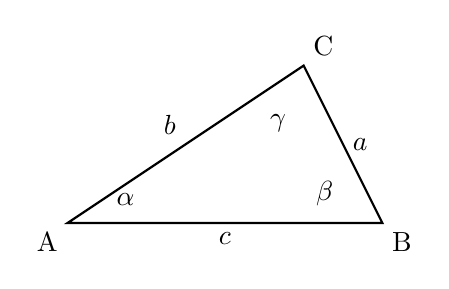
\begin{tikzpicture}

		% Define the points of the triangle
		\coordinate (A) at (0,0);
		\coordinate (B) at (4,0);
		\coordinate (C) at (3.0,2.0);
		
		% Draw the triangle
		\draw [thick] (A) -- (B) -- (C) -- cycle;
		
		% Mark the angles
		\centerarc[](A)(0.0:33.7:0.4)
		\node[above right= 0.1cm and 0.5cm of A] {$\alpha$};

		\centerarc[](B)(180.0:116.6:0.4)
		\node[above left= 0.1cm and 0.5cm of B] {$\beta$};

		\centerarc[](C)(213.7:296.6:0.4)
		\node[below left= 0.5cm and 0.1cm of C] {$\gamma$};

		% Label the vertices
		\node[below left] at (A) {A};
		\node[above right] at (C) {C};
		\node[below right] at (B) {B};

		% Label the sides
		\node (a) at ($(B)!0.5!(C)$) [anchor=west] {$a$};
		\node (b) at ($(A)!0.5!(C)$) [anchor=south east] {$b$};
		\node (c) at ($(A)!0.5!(B)$) [anchor=north] {$c$};
		
	\end{tikzpicture}
	
	\subsection{Rechtwinkliges Dreieck}
	
	a: Ankathete von $\beta$, Gegenkathete von $\alpha$\\
	b: Ankathete von $\alpha$, Gegenkathete von $\beta$\\
	c: Hypotenuse \\
	
	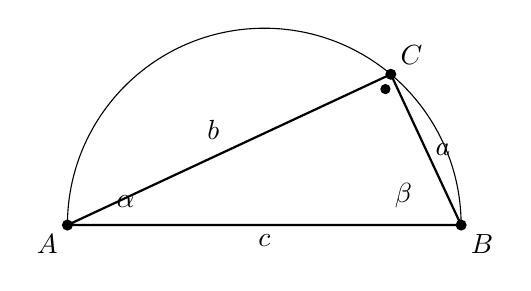
\begin{tikzpicture}
		
		% Define the points A, B (endpoints of the diameter)
		\coordinate (A) at (0, 0);
		\coordinate (B) at (5, 0);
		
		% Define the midpoint M
		\coordinate (M) at ($(A)!0.5!(B)$);
		
		% Define point C on the semicircle
		\coordinate (C) at ($(M) + (50:2.5cm)$);  % Angle 50 degrees from the horizontal
		
		% Draw the semicircle
		\draw[] (A) arc[start angle=180, end angle=0, radius=2.5cm];
		
		% Draw the diameter
		\draw[thick] (A) -- (B);
		
		% Draw right-angled triangle
		\draw[thick] (A) -- (C) -- (B) -- cycle;

		% Mark the points A, B, C
		\fill[black] (A) circle (2pt) node[below left] {$A$};
		\fill[black] (B) circle (2pt) node[below right] {$B$};
		\fill[black] (C) circle (2pt) node[above right] {$C$};

		% Draw angle arcs and labels
		\centerarc[](A)(0:25:0.4)
		\node[above right= 0.1cm and 0.5cm of A] {$\alpha$};

		\centerarc[](B)(180:115:0.4)
		\node[above left= 0.1cm and 0.5cm of B] {$\beta$};

		% Right angle dot
		\centerarc[](C)(205:295:0.4)
		\draw[thick,fill=black] ($(C) + (250:0.2)$) circle[radius=0.05];

		\node at ($(A)!0.5!(C)$) [anchor=south east] {$b$};
		\node at ($(B)!0.5!(C)$) [anchor=west] {$a$};
		\node at ($(A)!0.5!(B)$) [below] {$c$};
		
	\end{tikzpicture}

	\subsection{Sinus und Cosinus}
		Der Sinus ist eine ungerade Funktion \\
		Der Cosinus ist eine gerade Funktion
		\begin{emphbox}
			\begin{align*}
				\sin(\alpha) &= \frac{a}{c} = \cos(\beta) \\
				\sin(\beta) &= \frac{b}{c} = \cos(\alpha)
			\end{align*}
		\end{emphbox}

	\subsection{Symmetrieeigenschaften}
		\begin{emphbox}
			\begin{align*}
			\sin (-\alpha) &= -\sin(\alpha) \\
			\sin (90 \degree + \alpha) &= \sin (90 \degree - \alpha) \\
			\cos (-\alpha) &= \cos(\alpha)\\
			\cos (90 \degree + \alpha) &= -\cos (90 \degree - \alpha)
			\end{align*}
		\end{emphbox}


	\subsection{Tangens}
		\begin{emphbox}
			\begin{align*}
			\tan(\alpha) &= \frac{a}{b} = \frac{\sin(\alpha)}{\cos(\alpha)} \\
			\tan(\beta) &= \frac{b}{a} = \frac{\sin(\beta)}{\cos(\beta)}
			\end{align*}
		\end{emphbox}
		
	\subsection{Cotangens}
		\begin{emphbox}
			\begin{align*}
			\cot(\alpha) &= \frac{1}{\tan(\alpha)} \\
			\cot \alpha &= \frac{\cos \alpha}{\sin \alpha} 		
			\end{align*}
		\end{emphbox}

	\subsection{Trigonometrischer Pythagoras}
		\begin{emphbox}
			$ \sin ^2 \alpha + \cos ^2 \alpha = 1 $
		\end{emphbox}
		
	\subsection{Sinussatz}
		\begin{emphbox}
			$ \frac{a}{\sin \alpha} = \frac{b}{\sin \beta} = \frac{c}{\sin \gamma} = \frac{a \cdot b \cdot c}{2 \cdot A} = 2 \cdot R$
		\end{emphbox}

	\subsection{Cosinussatz}
		\begin{emphbox}
			$ c^2 = a^2 + b^2 - 2 \cdot a \cdot b \cdot \cos \gamma $
		\end{emphbox}

\begin{symbolbox}
	A = Fläche\\
	R = Radius des Umkreises
\end{symbolbox}

\begin{bluebox}
	Test
\end{bluebox}


\end{sectionbox}


\begin{sectionbox}
	\subsection{Cosinus}

	Text goes here ...


\end{sectionbox}




% ======================================================================
% End
% ======================================================================
\end{document}
